\chapter{Fundamentals and Related Work}
\label{cha:Fundamentals}

This chapter would discuss the details of the various components involved highlighting
the use of the components for the completion of this thesis. The last section
would give a overview of related work which provide some details of systems which
are either partially related to this thesis or form the basis for the thesis to improve
upon.

\section{Nodal Discontinuous Galerkin Method}
\label{sec:dgtd}

The \ac{DGTD} \cite{hesthaven_nodal_2008} is used to find solutions
for partial differential equations (PDE) numerically. This method is efficient in
producing results with computers as it relies on mathematical calculations on elemental basis.
This allows to perform computation in parallel on similar or different hardware helping to
solve problems from different domains quickly. \ac{DGTD} method is particularly popular for applications
in the domains such as fluid mechanics, plasma physics and electrodynamics.

\subsection{DGTD to solve Maxwell equations}
\label{sec:dgtd_maxwell}

\textcite{Hesthaven_190449} presented the use of \ac{DGTD} to solve time-domain Maxwell's equations with
an 1D and 2D examples and the extension to 3D is explained in \cite{hesthaven_nodal_2008}. This section
would briefly describe the formulations and steps involved for getting the solutions which are
used as the basis for implementation in the application used in this thesis to simulate
electromagnetic flux values for a given material.

The basic equation involved in computation of the electromagnetic flux is Maxwell's equations. The
three dimensional time-dependent Maxwell's equations \cite{hesthaven_nodal_2008} is written as:
\begin{equation}\label{eqn:maxwellbase}
    \mu \frac{\partial{\textbf{H}}}{\partial{t}} = - \nabla \times \textbf{E},\varepsilon \frac{\partial{\textbf{E}}}{ \partial{t}} = - \nabla  \times \textbf{H}
\end{equation}
the conservation form of the equation can be expressed as:
\begin{equation}\label{eqn:maxwell}
    \mathcal{Q}\frac{\partial\textbf{q}}{\partial{t}}  + \nabla  \cdot \mathcal{F} = 0
\end{equation}
where
\begin{equation}\label{eqn:maxwellexpansion}
\textbf{q} =  \begin{bmatrix}\textbf{H} \\ \textbf{E} \end{bmatrix},
\mathcal{Q} =  \begin{bmatrix} \mu & 0 \\ 0 &  \varepsilon \end{bmatrix},
\mathcal{F} = \begin{bmatrix}  - \widehat{n} \times \textbf{E} \\ \widehat{n} \times \textbf{H} \end{bmatrix} = \begin{bmatrix} \textbf{F}_H \\ \textbf{F}_E \end{bmatrix}
\end{equation}

\textbf{H} and \textbf{E} are the magnetic and electric vector fields in
three dimensions which are function of the positional coordinates and time
$ (\tilde{x},\tilde{y}, \tilde{z}, \tilde{t}) $, $ \mathcal{Q} $ defines the magnetic permeability
$ \mu(x) $ and the electric permittivity $ \varepsilon(x) $ of the material.

Now considering that we have a object composed of a single type of material with known $ \mathcal{Q} $
values, the DG method can be used to solve the equation \ref{eqn:maxwell} by discretization of the
computation domain $ \Omega $ (whole of the object) spatially. In 3D, this can be achieved by dividing the object
into K tetrahedral elements and computing the local approximated solution $ u_h^k(x,t) $ for
each element $ D^k \in K $. This local solution is computed for a defined polynomial order $ N $ such that,
$ h \in N $ represents the $ h^{th} $ polynomial of $ D^k $ and is called the nodal point.
Now for a given polynomial order $ N $, the local solution can be expressed \cite{hesthaven_nodal_2008} as:
\begin{equation}\label{eqn:nodal_form}
    x \in D^k \ : \ u^k_{h}(\textbf{x}, t) \; = \; \sum_{n=1}^{N_p} \hat{u}_n(t) \psi_{n}(\textbf{x}) \; = \; \sum_{i=1}^{N_p} u^k_{h}(\textbf{x}_{i}, t) l^k_{i}(\textbf{x})
\end{equation}
where $ l^k_{i}(\textbf{x}) $ is the multidimensional Lagrange polynomial and $ \psi_{n}(\textbf{x}) $
is a three-dimensional polynomial basis.

In equation \ref{eqn:nodal_form}, the $ N_p $ denotes the number of nodal points per element $ D^k $
and depends on the polynomial order $ N $ which is given by:
\begin{equation}\label{eqn:nprelation}
    N_p = \frac{(N+1)(N+2)(N+3)}{6}
\end{equation}

Now that we know the basis for computation of local approximated solutions,
the next step is to compute the global solution, which can be achieved by summing
up the these individual solutions $ u_h^k(x,t) $ except for nodal points on the faces.
The nodal points on the faces of the tetrahedra would have two different solution
as they can be part of two different $ D^k $ elements and required coupling of the
solution. The coupling of the solution is done by computing the electric and
magnetic field differences \cite{kenter_opencl-based_2018} $\Delta \textbf{E}
= \textbf{E}^+-\textbf{E}^-, \Delta \textbf{H} = \textbf{H}^+ - \textbf{H}^-$.
Combining the local and the global solutions is achieved \cite{kenter_opencl-based_2018, busch_discontinuous_2011}
by a pair of \ac{ODE} for the semi-discrete system derivation or which is explained in
\cite{hesthaven_nodal_2008}:
\begin{equation}\label{eqn:pde_e}
\epsilon^k \frac{\partial \textbf{E}^k}{\partial t} = \textbf{D}^k \times \textbf{H}^k
+ (\mathcal{M}^k)^{-1}\mathcal{F}^k \left( \frac{\Delta\textbf{E}-\hat{n} \cdot (\hat{n} \cdot \Delta \textbf{E})+Z^+ \hat{n} \times \Delta \textbf{H} }{\overline{Z}} \right)
\end{equation}
\begin{equation}\label{eqn:pde_h}
    \mu^k \frac{\partial \textbf{H}^k}{\partial t} = - \textbf{D}^k \times \textbf{E}^k
    + (\mathcal{M}^k)^{-1} \mathcal{F}^k \left ( \frac{\Delta \textbf{H} -\hat{n} \cdot (\hat{n} \cdot \Delta \textbf{H})-Y^+ \hat{n} \times \Delta \textbf{E}}{\overline{Y}} \right)
\end{equation}
where $ (\mathcal{M}^k) $ is mass matrix, $\mathcal{F}^k$ is face matrix, $\hat{n}$ outwardly
pointing normal vector to the element face where the flux is calculated. The $ Z^\pm $ and $Y^\pm$ is the impedance and the conductance of the material.

The solution of these \ac{ODE}s require time discretization. The Runge-Kutta
scheme introduced in \cite{shu_total-variation-diminishing_1988} is used
\cite{hesthaven_nodal_2008, kenter_opencl-based_2018} to integrate the
equations in time. The timesteps are chosen in way such that they are small
and ensure that the timestep error can be neglected. In the implementation used
in this thesis, the timestep is computed by calculating the smallest distance between two nodal points.

\section{\acf{MIDG2}}

\ac{MIDG2} is a open source C/C++ based application which implements the \ac{DGTD} method for solving
Maxwell's equations for 1D, 2D and 3D. It uses K non-overlapping tetrahedra elements as described in
section \ref{sec:dgtd_maxwell} for computing the flux values for a given object. This section
will give an overview of the application implementation along with improvements done to use
multiple FPGAs to offload the computation and speed up the execution time.

The original MIDG2 implementation supports parallelization using \ac{MPI} for multiple CPUs and
uses OCCA \footnote{\url{https://libocca.org}} to provide support for acceleration with GPU
using CUDA and OpenCL™. The object for which the flux is to be computed is represented as
an unstructured mesh of K non-overlapping tetrahedral elements as shown in fig \ref{fig:mesh}.
This mesh is generated using the tool Tetgen\footnote{\url{http://wias-berlin.de/software/tetgen/}}
which is an open source tool to generate meshes. The tetrahedra within the mesh are
identified with their vertices. The application uses three vectors VX, VY and VZ
to store the coordinates of each of the vertices. The application performs the steps
which are formulated in section \ref{sec:dgtd_maxwell} using mesh and additional
inputs which include mass matrixes and Runge-kutta time step constants to compute the
flux values for a given polynomial order.
\begin{figure}[h]%
    \centering
    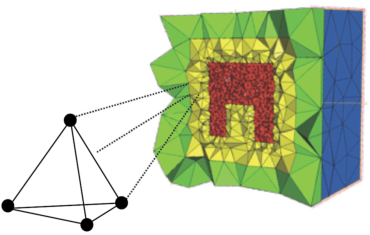
\includegraphics[width=0.6\textwidth]{images/mesh}
    \caption{K element mesh with tetrahedra elements for split-ring resonator object}
    \label{fig:mesh}
\end{figure}

The parallelization or computation can be achieved in this implementation by dividing
the mesh into partitions. As the \ac{DGTD} algorithm works by first computing individual
local solution for the elements and then accumulating the values over all $k's$,
a partitioning scheme which uses surfaces as boundaries can be performed such that,
computation of each individual partition is performed by a separate
process/thread/core/system and the shared surface data is shared at each time step
between them using a communication infrastructure. The partitioning in MIDG2 is
achieved using an open source tool ParMETIS\footnote{\url{http://glaros.dtc.umn.edu/gkhome/metis/parmetis/overview}},
which is effective in partitioning meshes for a distributed system for equal load sharing.
The MIDG2 uses \ac{MPI} for implementing a distribution and communication scheme which
allows to use multiple systems with distributed load to speedup the computation.
The whole process for partitioning and distribution is shown in fig \ref{fig:partitioning}.
\begin{figure}[h]%
    \centering
    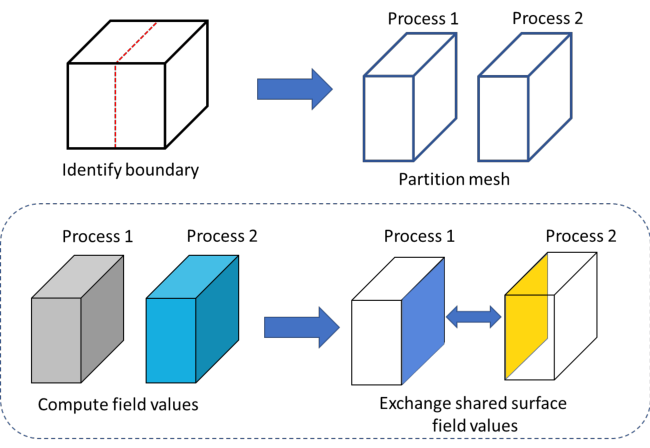
\includegraphics[width=0.9\textwidth]{images/partition_proc}
    \caption{Parallelization achieved with partitioning and processing by multiple processes}
    \label{fig:partitioning}
\end{figure}

\subsection{FPGA implementation for DGTD}
\label{sec:fpga_dg}

\textcite{kenter_opencl-based_2018} extended the original MIDG2 implementation to use
FPGAs to accelerate the computation for a single FPGA system. This implementation
uses Intel™ FPGA SDK for OpenCL™ to implement three compute kernels viz. volume kernel,
surface kernel and RK kernel which perform the computation steps for the \ac{DG} solver.
The kernels developed were optimized to utilize the capabilities of the FPGA such
as parallelization of operations by replication, optimizing memory access by using
local memory for storing constant data, using memory banks to allow parallel data
reads/writes for higher bandwidth lower stalls.
The structure of the OpenCL™ kernels for this implementation is shown in figure.
The IO kernels for surface and volume act as memory interface kernels which
access the global memory as source and sink for data. Use for multiple
kernels in such way along with the Intel™ FPGA OpenCL™
channels, create a pipeline structure for the volume and surface compute kernels
which allows to start computation on a nodal point in each cycle. The kernel
structure of the implementation is shown in figure \ref{fig:singlefpga_kernstruc}
which shows pipeline structure developed for acceleration with the single FPGA.
The complete implementation details along with performance evaluation for the design
is described in \cite{kenter_opencl-based_2018}.

\begin{figure}[h]%
    \centering
    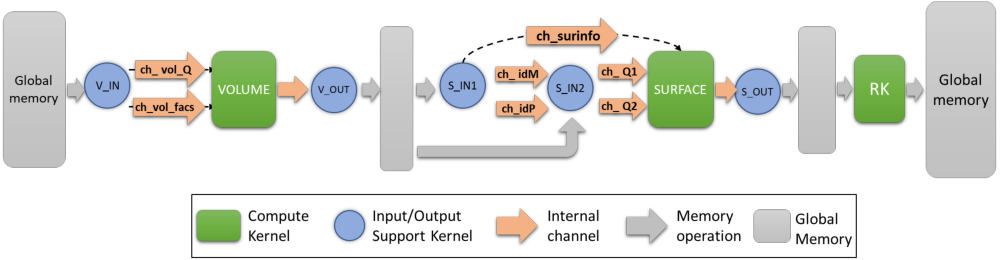
\includegraphics[width=1.0\textwidth]{images/nb_kernstruc}
    \caption{Block level structure for OpenCL™ kernels developed for single FPGA by \textcite{kenter_opencl-based_2018}}
    \label{fig:singlefpga_kernstruc}
\end{figure}

Further improvements to this design was made by extending the capabilities to work
with multiple FPGAs along with \ac{MPI}. The \ac{MPI} FPGA design works similar to the original
MIDG2 \ac{MPI} implementation. The mesh is divided into partitions using ParMETIS and
the computation is performed on different compute nodes of a cluster. The nodes
in this case also include the FPGAs which is used to offload the computing and
use the kernels from the FPGA based design. An additional kernel is introduced in
this design which is responsible to read the shared data and store it in a coalesced
memory. The host processor then reads this data from the FPGA memory and uses
\ac{MPI} to communicate with other nodes to which the data is shared. Figure
\ref{fig:mpi_fpga} shows the system architecture of this design.

\begin{figure}[h]%
    \centering
    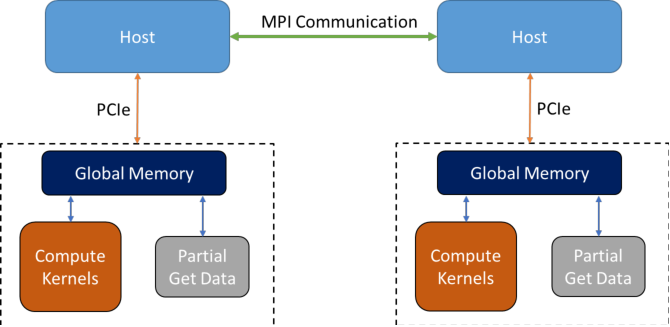
\includegraphics[width=0.9\textwidth]{images/mpi_fpga}
    \caption{System level architecture for MPI FPGA design communicating using MPI and PCIe}
    \label{fig:mpi_fpga}
\end{figure}

Using this design multiple FPGAs can be used to speed up the computing even further.
Though speed ups can be achieved with this design, the communication which involves
movement of data through \ac{PCIe} bus and the network interface two times,
reduces the communication bandwidth a lot. This communication setup also
requires to have synchronization constructs between the FPGA and the host
processor to ensure data correctness which adds a lot of overhead in the overall
execution time. This thesis uses this design as the base versions and replaces
the communication with point-to-point communication between FPGAs which allows
removing the complex communication and synchronization steps and speed up the
execution even further.

\section{Hardware and Software Platform}

This section would describe the hardware and the software platform used in the
thesis for implementing and evaluating the extended design. The first subsection
gives an overview of Nallatech 520N board followed by and description of software
setup using Intel™ FPGA SDK for OpenCL™ used to implement the kernels for the
features.

\subsection{Nallatech 520N}

The Nallatech 520N boards used for the evaluation are equipped with

\begin{enumerate}
    \item Intel™ Stratix 10 FPGA GX2800 capable for providing up to 10 TFLOPS of single
    precision floating point performance
    \item DDR4 SDRAM memory divided into 4 banks with 8GB each giving a total memory of 32GB with
    a transfer rate of 2400 MT/s
    \item Four 100/40/25/10G QSFP28 Network Ports
    \item 16-lane PCI-Express Gen 3.0 for high speed host to FPGA data transfers
\end{enumerate}

The Intel™ Stratix 10 FPGA GX2800 FPGA belongs to the current generation of the high-performance FPGA
family with new Intel™ Hyperflex™ core architecture which gives higher bandwidth and processing
performance to the FPGAs. The resource summary for the FPGA is given in table \todo{add table}
which shows the high computation capabilities of the FPGAs

\subsubsection*{QSFP Network Ports}

Along with huge processing power, the Nallatech board also contains 4 QSFP Network Ports which
are connected to the FPGA transceivers to provide high speed network communication. As mentioned
previously these ports are used in this thesis to setup FPGA-to-FPGA networks to transfers data
and reduce communication latency. The connections in the used setup are done using
Finisar's FTL410QE2C and Edge's FTL410QE3C QSFP+ optical transceivers modules which support a
maximum link length of 150 meters. The maximum data rate varies from 39.8 Gbits/s to 44.8 Gbits/s.
As the Nallatech BSP supports 40 Gbits/s speeds, this is used for all calculation in this thesis.


\subsection{Software Development flow}

Intel™ FPGA SDK for OpenCL™ is used for the extending the existing kernels.
\TODO{GIve details after finalizing}

\subsection{OpenCL™ Serial IO channels}

The communication over the QSFP ports can be implemented in the OpenCL™ by using the
Intel's OpenCL™ IO channels support. The IO channels can be used to stream data
directly between kernels and I/O using explicitly named channels. The declaration
of these channels should be included in the \texttt{board\_spec.xml} using the
\texttt{channels} element. The Nallatech BSP provide 4 Tx and 4 Rx IO channels for the 520N board
as shown in the listing {} which interface to the 4 QSFP ports on the board.
In order to use these I/O channels in the OpenCL kernel,
an \texttt{io} attribute is included in the channel declaration along with id of
the interface which is specified in the \texttt{board\_spec.xml}.

\TODO{Revise the introduction of the IO channels to describe that is it provided by Nallatech}
\begin{XmlCode}
<channels>
    <interface name="board" port="io_to_dev_ch0" type="streamsource" width="256" chan_id="kernel_input_ch0"/>
    <interface name="board" port="dev_to_io_ch0" type="streamsink" width="256" chan_id="kernel_output_ch0"/>
    <interface name="board" port="io_to_dev_ch1" type="streamsource" width="256" chan_id="kernel_input_ch1"/>
    <interface name="board" port="dev_to_io_ch1" type="streamsink" width="256" chan_id="kernel_output_ch1"/>
    <interface name="board" port="io_to_dev_ch2" type="streamsource" width="256" chan_id="kernel_input_ch2"/>
    <interface name="board" port="dev_to_io_ch2" type="streamsink" width="256" chan_id="kernel_output_ch2"/>
    <interface name="board" port="io_to_dev_ch3" type="streamsource" width="256" chan_id="kernel_input_ch3"/>
    <interface name="board" port="dev_to_io_ch3" type="streamsink" width="256" chan_id="kernel_output_ch3"/>
</channels>
\end{XmlCode}
A example kernel code is shown in the listing {} which uses one TX and one RX channel to
communicate in the \texttt{sender} and \texttt{collector}.
\texttt{ch\_eth\_in} and \texttt{ch\_eth\_out} is declared to interface with
the external channels \texttt{kernel\_input\_ch0} and \texttt{kernel\_output\_ch0} respectively.
The channels should be declared with a datatype (\texttt{float8} in this case)
suitable to hold the 256 bits wide data which is the current width of the channels.
After the declaration, the channels can be used by the kernel similar to standard OpenCL™
channels using \texttt{write\_channel\_intel} and \texttt{read\_channel\_intel} APIs to write
to the TX channel and read from the RX channel as shown.

\begin{CppCode}
#pragma OPENCL EXTENSION cl_intel_channels : enable

channel float8 ch_eth_in __attribute((io("kernel_input_ch0")));
channel float8 ch_eth_out __attribute((io("kernel_output_ch0")));

__kernel void __attribute__ ((max_global_work_dim(0)))
sender(int length, __global float8 * restrict input)
{

    for(int i=0; i<length; ++i)
        write_channel_intel(ch_eth_out, input[i]);


}

__kernel void __attribute__ ((max_global_work_dim(0)))
collector(int length, __global float8 * restrict output)
{

    for(int i=0; i<length; ++i)
        output[i] = read_channel_intel(ch_eth_in);

}
\end{CppCode}


\TODO{Add section to describe loop pipeline in nexted loops}
\TODO{Add section to describe Memory banking and benfits in OpenCL™ kernels}

